For $z\lesssim 2$, a large fraction of the predicted baryon content is missing in observations. The majority of these baryons are believed to reside in the warm-hot intergalactic medium (WHIM), with typical temperatures of $10^5$ K to $10^7$ K \cite{Pen1999,Soltan06}. Its high temperature and associated low density impose difficulties for direct detection. Furthermore, the uncertainty in the spatial distribution of its ionization state, metalicity, and pressure lead to confusion in interpreting signals from absroption lines and soft X-rays. There is therefore an urgency for probes that not only trace the majority of the missing baryons, but also can be interpreted model-independently.

Among proposed probes, the kinematic Sunyaev-Zel'dovich (kSZ) effect \cite{Sunyaev72,Sunyaev80,Vishniac87} is a promising one. The kSZ effect results from Compton scattering of Cosmic Microwave Background (CMB) photons off of free electrons. The radial velocity of the electrons provides a Doppler shift to the photons causing a secondary anisotropy in CMB temperature. 
%The kSZ signal could satisfy all three conditions listed before. 
%Consider kSZ as tracer has lots of advantages for this problem. 
It is an ideal probe to tackle the missing baryon problem: First, it recieves a contribution from all the free electrons. 
%in all temperature and dynamic range. 
For low redshift, $\gtrsim 90\%$ of baryons are in ionized states \cite{Fukugita04}, 
and can be traced by free electrons. %First, it contributes from all the free electrons, indicating the distribution of $90\%$ of the baryons in ionized states,   
%leaving alone only less than $10\%$ of baryons that 
%reside in stars, remnants, atomic and molecular gases \cite{Fukugita04}. 
%
Second, the signal is mainly influenced by the electron density and radial velocity, regardless of the temperature, pressure, and metalicity, so no extra assumptions are needed to estimate the baryon abundance. Third, the dominant piece of the peculiar velocity signal comes from the large-scale structure, and therefore the signal is less biased by the local environment, and more indicative of the diffuse distribution.

Attractive as it is, two drawbacks largely reduce the feasibility of harnessing the kSZ signal. First, the signal is weak compared to the primary CMB anisotropies and hence suffers seriously from contaminations from the primary, instrumental noise, the thermal SZ effect, CMB lensing, etc \dots Second, it is an integrated effect along the line of sight and does not contain redshift information.

Cross correlation of the kSZ signal with another tracer, which has both large-scale structure and redshift information, provides a straight-forward mitigation of these disadvantages. Previous work has proposed optical spectroscopic surveys as an ideal tool \cite{Hand12,Shao11,Li14}. 
%However, lack of spectral lines in redshift $1.4-2.5$, and low survey speed has limited the application.
However, the lack of prominent spectral lines at redshift $1.4-2.5$ makes it difficult to consistently measure evolution from $z=2$ to $z=0$. 
%And kSZ signal is more prominent at $z\sim2$ than $z<1.4$, 
%making it painful to leave out this stretch.
Moreover, the difficult technical specifications required for source detection, especially at high redshift, largely constrain the sky coverage and limit such surveys to relatively small angular scales, where the power from the primary CMB is low. Methods with lower requirements on facilities such as cross-correlation of photo-z galaxies with kSZ \cite{Hill16,Ferraro16}, depend on models of velocity fields and demand next generation CMB facilities, such as ACTpol, CMB-S4, to achieve convincing S/N.
%Optical spectroscopic surveys have been proposed as an ideal candidate. 
%Opitical spectroscopic surveys are one popular candidate. 
%However, they are not accessible on redshift $1.4-2.5$ 
%when all the lines are shifted away. 
%To consistently measure the sky from $z=0$ to $z=2$, we consider harness the H~I $21$ cm  line in radio band, which can also provide accurate redshift information.
%Rather than distinguishing individual galaxies, 
%we discuss the possibility of using integrated signals of each pixel 
%(intensity mapping) 

In this paper, the new possibility of cross-correlating the neutral hydrogen (HI) density field from 21 cm intensity mapping (IM) experiments with the kSZ signal is discussed and tested with simulations. The redshifted 21 cm line provides accurate redshift information, which will soon be available at $z\lesssim2$.  
%which enables us to reconstruct velocity field and 
%get better correlation with kSZ powerspectra. 
Intensity mapping surveys, rather than distinguishing individual galaxies, integrate all signals in a pixel, enabling them quickly scan large areas of the sky. In the following few years, there will be several full-sky experiments producing data at redshifts $\lesssim2.5$ 
\cite{2014CHIME, TIANLAI, HIRAX}.
With the abundant data of density fields with accurate redshift information, we are able to linearly reconstruct the velocity fields, and hence calculate a 
large sky kSZ map to cross correlate with real kSZ signals. 

Promising as it seems, the loss of large-scale modes in IM surveys will complicate the cross-correlation of the IM field with kSZ signals. The main challenge comes from the bright astrophysical foregrounds, which contaminate the large-scale modes parallel to the line of sight, i.e. small $k_\parallel$ modes. Besides, the large-scale modes in perpendicular plane, i.e. small $k_\perp$ modes, is poorly resolved with inteferometers. Fig.\ref{fig:cmb_21cm} shows an illustration of the modes of the matter density field which can be observed by a CHIME-like survey.
%Consider the contamination from promary CMB 
%and noise scale of Planck
Since the large scale modes are essential 
for calculating velocity fields, 
directly using this IM fields to cross correlate with kSZ signal can only 
resolve $<20\%$ of the signal.  

Therefore, in this work, 
we first solve for the large-scale modes 
from their non-linear tidal distortions on small scale power spectrum \cite{2012:pen,2015:zhu}. 
As shown in simulations, velocity fields can be well reproduced 
after the algorithm. 
Convolving the reconstructed $v_z$ with large $\ell$ density fields, we could better assemble observable kSZ signals. 
The full procedure is depicted at the bottom of Fig. \ref{fig:cmb_21cm}. 
The effect on the cross-correlation obtained from this method of varying various survey-related parameters such as foreground noise level, shortest baseline length, spatial and frequency resolution are discussed.

The paper is organized as follows: Section II introduces the method we use to cross-correlate density fields with the kSZ signal (similarly to \cite{Shao11}); Section III discusses the realities of 21cm IM surveys and properties of the observed fields; Section IV clarifies the important scales of the density and velocity fields in relation to the kSZ signal; Section IV describes the non-linear tidal reconstruction method for the missing large-scale modes in the IM fields; Section V presents our analytical and numerical results, while in Section VI we summarize our S/N calculations; We conclude in Section VII.

\begin{figure}[tbp]
\begin{minipage}[t]{\linewidth}
\vspace{-0.8cm}
\includegraphics[width=\textwidth]{figure/cmb_21cm.eps}
\vspace{-0.6cm}
\label{fig:cmb_21cm}
\end{minipage}
\begin{minipage}[t]{\linewidth}
\vspace{-0.8cm}
\includegraphics[width=\textwidth]{figure/demo_convolution.eps}
\vspace{-0.6cm}
\end{minipage}
\caption{
%    All the $k$ and $\ell$ are matched for $z=1$
(Top) Theoretical prediction for the two-dimensional power spectrum of 21 cm fluctuations at $z=1$ observed by CHIME, assuming high foregrounds ($R_\parallel=15$ h/Mpc). See discussions in Section.\ref{sec:21cm}. (Middle) Window for kSZ measurements based on Planck 217 GHz band noise. The kSZ signal is calculated in 1.2 Gpc boxes.
%Demonstration of cross correlation algorithm, 
(Bottom) The algorithm first solve for the lost large scale modes 
with tidal reconstruction 
and use it to calculate velocity fields.   
The kSZ signal is a convolution of density and velocity in Fourier space, 
therefore velocity and density fields of different k are coupled together 
as discussed in Section.\ref{sec:kszAnalysis}. 
\philnote{See figure 9 in https://arxiv.org/pdf/1401.2095v1.pdf }
}
\end{figure}
